%!TEX root = ../thesis.tex
%*******************************************************************************
%*********************************** Third Chapter *****************************
%*******************************************************************************
\chapter{Kernel-based uncertainty quantification}
%*******************************************************************************
\hfill
\localtableofcontents
\newpage

\elias{Star by the second part}
%============================================================%
\section{Introduction}
%============================================================%



\elias{Copulogram: a graphical tool for visulazing multivariate datasets.}
\elias{Have a paragraph in the introduction that refers to the appendix.}


%============================================================%
\section{Nonparametric fit of the environmental inputs}\label{sec:32_inference}
%============================================================%

\elias{If Alexis scripts work: compare the adequancy between the two strategies using the MMD for increasing sample sizes. }

\subsection{Marginal inference}
%============================================================%



\subsection{Conditional model to infer the dependence}
%============================================================%



\subsection{Empirical copula model to infer the dependence}
%============================================================%





%============================================================%
\section{Quantifying and clustering the wake-induced perturbations within a wind farm}
%============================================================%

\elias{add ref: ``Difference in load predictions obtained with effective
turbulence vs. a dynamic wake meandering
modeling approach''}


In the offshore wind industry, the wake effect is considered crucial for electricity production and structural fatigue of turbine components. 
For instance, the standards developed by the International Electrotechnical Commission (see appendix E in \cite{IEC61400-1}) review some analytical \cite{Frandsen2007}, and numerical models (e.g., the dynamic wake meandering approach by \cite{Larsen2008}) to simulate the wind speed deficit and the wake added turbulence. 
Since the pioneering work of \cite{Jensen1983}, several wake models were developed and compared in a benchmark by \cite{Doubrawa2020}. 
This work takes advantage of the low computational cost of steady-state wake models to propagate the uncertainty from ambient to wake-induced wind conditions seen on a farm. 
It is worth noting that the wake creates a heterogeneous wind field in a wind farm, resulting in different loading conditions which should be considered at the stage of reliability based design (RBD). 
Such heterogeneity is not taken into account by the design load cases of international standards (see e.g., \cite{IEC61400-1,DNV-OS-J103}) where wind and wave conditions are derived from scenarios occurring over long-term periods. 
Wake models allow us to simulate the wind conditions' distribution at each turbine, however, the RBD step is too costly to be performed for each turbine. 
For further details regarding the RBD, one may refer to the work of \cite{huchet_2019, slot_sorensen_2020, stieng_muskulus_2020, wilkie_galasso_2021}, proposing several approaches to reduce the computational cost of this step. 
In order to speed up the RBD at the scale of a wind farm, the present work aims at building clusters of WT similarly affected by the wake. 
Then, the RBD over a wind farm can be computed only on a few WT, each representing a cluster of turbines enduring similar wake-modified wind loading. This clustering is done on two wind parameters, following the conclusions of the global sensitivity analysis of \cite{McWilliam2022}. 
In order to discriminate the wake-perturbed distributions of wind parameters, the maximum mean discrepancy (MMD) is used as a statistical metric between multivariate distributions (as reviewed by \cite{Sriperumbudur2010}). 
To illustrate this novel approach, a theoretical wind farm for the ongoing tenders off the coast of South Brittany in France is studied, with a modified version of the floating offshore wind turbine (FOWT) IEA-15MW (initially proposed in \cite{Allen2020,Gaertner2020}). 
Figure~\ref{fig:SB-farm} illustrates the layout of the 25 FOWT considered in the following. 
This layout is regular with an inter-turbine distance of seven times the rotor diameter in the dominant wind direction and five times the rotor diameter in the orthogonal (crosswind) direction. 
More details regarding the FOWT modifications and theoretical wind farm can be found in \cite{Capaldo2021,Peyrard2022}.

\begin{figure}[h]
\centering
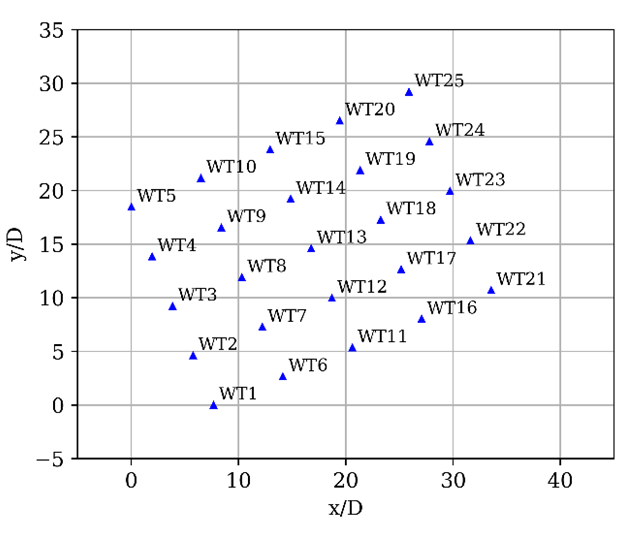
\includegraphics[width=15pc]{part2/figures/WAKE/SB1.png}
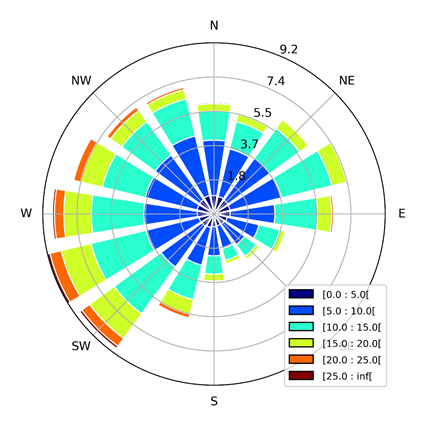
\includegraphics[width=13pc]{part2/figures/WAKE/SB2.png}\hspace{2pc}
\caption{\label{fig:SB-farm} 
South Brittany wind farm layout (left). South Brittany wind rose from the ANEMOC data (right, source: \cite{Ardillon2023}).}
\end{figure}

Based on the results of previous numerical studies, with either dynamic wake meandering \cite{Wise2020} or LES \cite{Johlas2021}, we retain the time-averaged floater position (translation and rotation) as the main effect of the floater motion on the far wake. It was shown that this effect is small, both on the wake-added turbulence and on the wind speed deficit. However, noticeable uplift of the wake may influence the fatigue design. 

The key idea in this paper to reduce the number of cases for RBD is to employ clustering techniques on the wake-induced wind parameters, to constitute groups of WT that are exposed to similar design load conditions. To do so, the present work is divided into four sections. First, the wake model used in this work is presented in section~\ref{sec:farmshadow}. Then, section~\ref{sec:UQ-wake} describes the uncertainty propagation through the wake model, from the probabilistic distribution of ambient wind parameters to the wake-modified wind parameters distribution within the farm. In order to regroup the similar wake-modified distributions, an adapted statistical metric on multivariate distributions is introduced in section~\ref{sec:metric}. Finally, the application of several clustering methods to the South Brittany case study is compared in section~\ref{sec:clustering}. The main conclusion suggests four clusters among the 25 FOWT which can then be used for RBD analysis of the farm.


%------------------------------------------------------------%
\subsection{Uncertainty propagation in a wake model}
\label{sec:UQ-wake}
%------------------------------------------------------------%
The wake model described in section~\ref{sec:farmshadow} takes as input a set of variables describing the ambient wind conditions $\bx \in \mathbb{R}^3$ and computes the perturbed wind conditions at each WT represented by the vector $\bx _l', l \in (1,..,n_{WT})$, where $n_{WT}$ is the total number of turbines in the farm:
\begin{align}
    g:\mathbb{R}^3 &\rightarrow \mathbb{R}^{3 n_{WT}} \\
    \bx &\longmapsto g(\bx) = (\bx_1',..,\bx_{n_{WT}}')
\end{align}
The uncertainties associated with the ambient wind conditions are represented by a random vector $\bX$ following the distribution $p_0$. 
Note that the index 0 is a reference to the fact that these conditions are not perturbed by the wake. 
A parametric model has been fitted in \cite{vanem_fekhari_2023} using conditional probability density functions to capture the dependence structure, with an approach similar to the one presented in~\cite{kelly_2022}. 
The random vector $\bX$ is described by the following input random variables:
\begin{itemize}
    \item Mean wind speed ($u$) is the 10-min average horizontal wind speed at hub height.
    \item Wind turbulence intensity ($TI$) is the 10-min wind speed turbulence intensity at hub height.
    \item Wind direction ($\theta$) is the 10-min average wind direction.
\end{itemize}
In the following, we assume the wind orientation variable $\theta$ to be unaffected by the wake. 
When perturbed by the wake of the wind farm, the WT~$l$ sees a wind flow represented by the random vector $\bX_l',l \in (1,..,n_{WT})$, following the distribution $p_l'$. 
Then, the two remaining parameters are $u_{rotor}$ and $TI_{rotor}$ to represent this modified wind flow on a vertical plane located at each WT. 
These two quantities of interest are averaged over the rotor while the input parameters are given at hub height. For the sake of simplicity, we will neglect this difference in what follows in order to consider the transformation $\bX'=g(\bX)$ as a simple perturbation of $\bX$. We will abusively denote $u$ and $TI$ both the input and output quantities. 
The output of the uncertainty propagation is a set of perturbed environmental distributions $p_l',l \in (1,..,n_{WT})$.
A Monte-Carlo sample $\bX_n={\bx^{(1)},..,\bx^{(n)}}$ of the three random input variables is generated. 
Then, considering the farm layout illustrated in Figure~\ref{fig:SB-farm} and a constant wind shear exponent of 0.1 like in section~\ref{sec:farmshadow}, a wake simulation is run for every wind condition of the Monte Carlo design of experiments. 
The code output consists in a multivariate joint distribution of modified $u$ and $TI$ for each WT. As the Monte Carlo procedure is known to converge slowly but surely, it was chosen to perform this uncertainty propagation with a number of simulations of size $n=6~000$ because of its simplicity and the low computational cost of the simulations.

 We can plot a preview of the wake perturbations on the joint distribution for given WT in the two dimensions $u$ and $TI$. 
 Figure~\ref{fig:FIGJointPerturbationSB} illustrates this perturbation for three WT differently affected by the wake depending on their position in the farm (cf. Figure~\ref{fig:SB-farm}). 
 One can notice that the WT~25 distribution (in orange) is very close to the ambient distribution (in black), as expected, this WT being located on the edge of the farm and facing the dominant wind direction. 
 Meanwhile, the WT~13 distribution (in red) seems more affected by the wake, by getting a higher wind turbulence with lower wind speed. 
 This analysis can be completed with the two marginals in Figure~\ref{FIGMarginalWSP} and Figure~\ref{FIGMarginalTI}, both describing the ambient marginal distributions (in black) and wake-disturbed distributions. 
 In general, a small wind speed deficit is noticed as indicated by the small shifts of the probability density functions to the left on Figure~\ref{FIGMarginalWSP}. 
 Also, a small added turbulence is indicated by the small shifts of the curves to the right on Figure~\ref{FIGMarginalTI}. 
 Ideally, a tool should allow us to quantify the perturbation between the ambient and perturbed distributions.

\begin{figure}
    \centering
    \begin{subfigure}[b]{0.3\textwidth}
        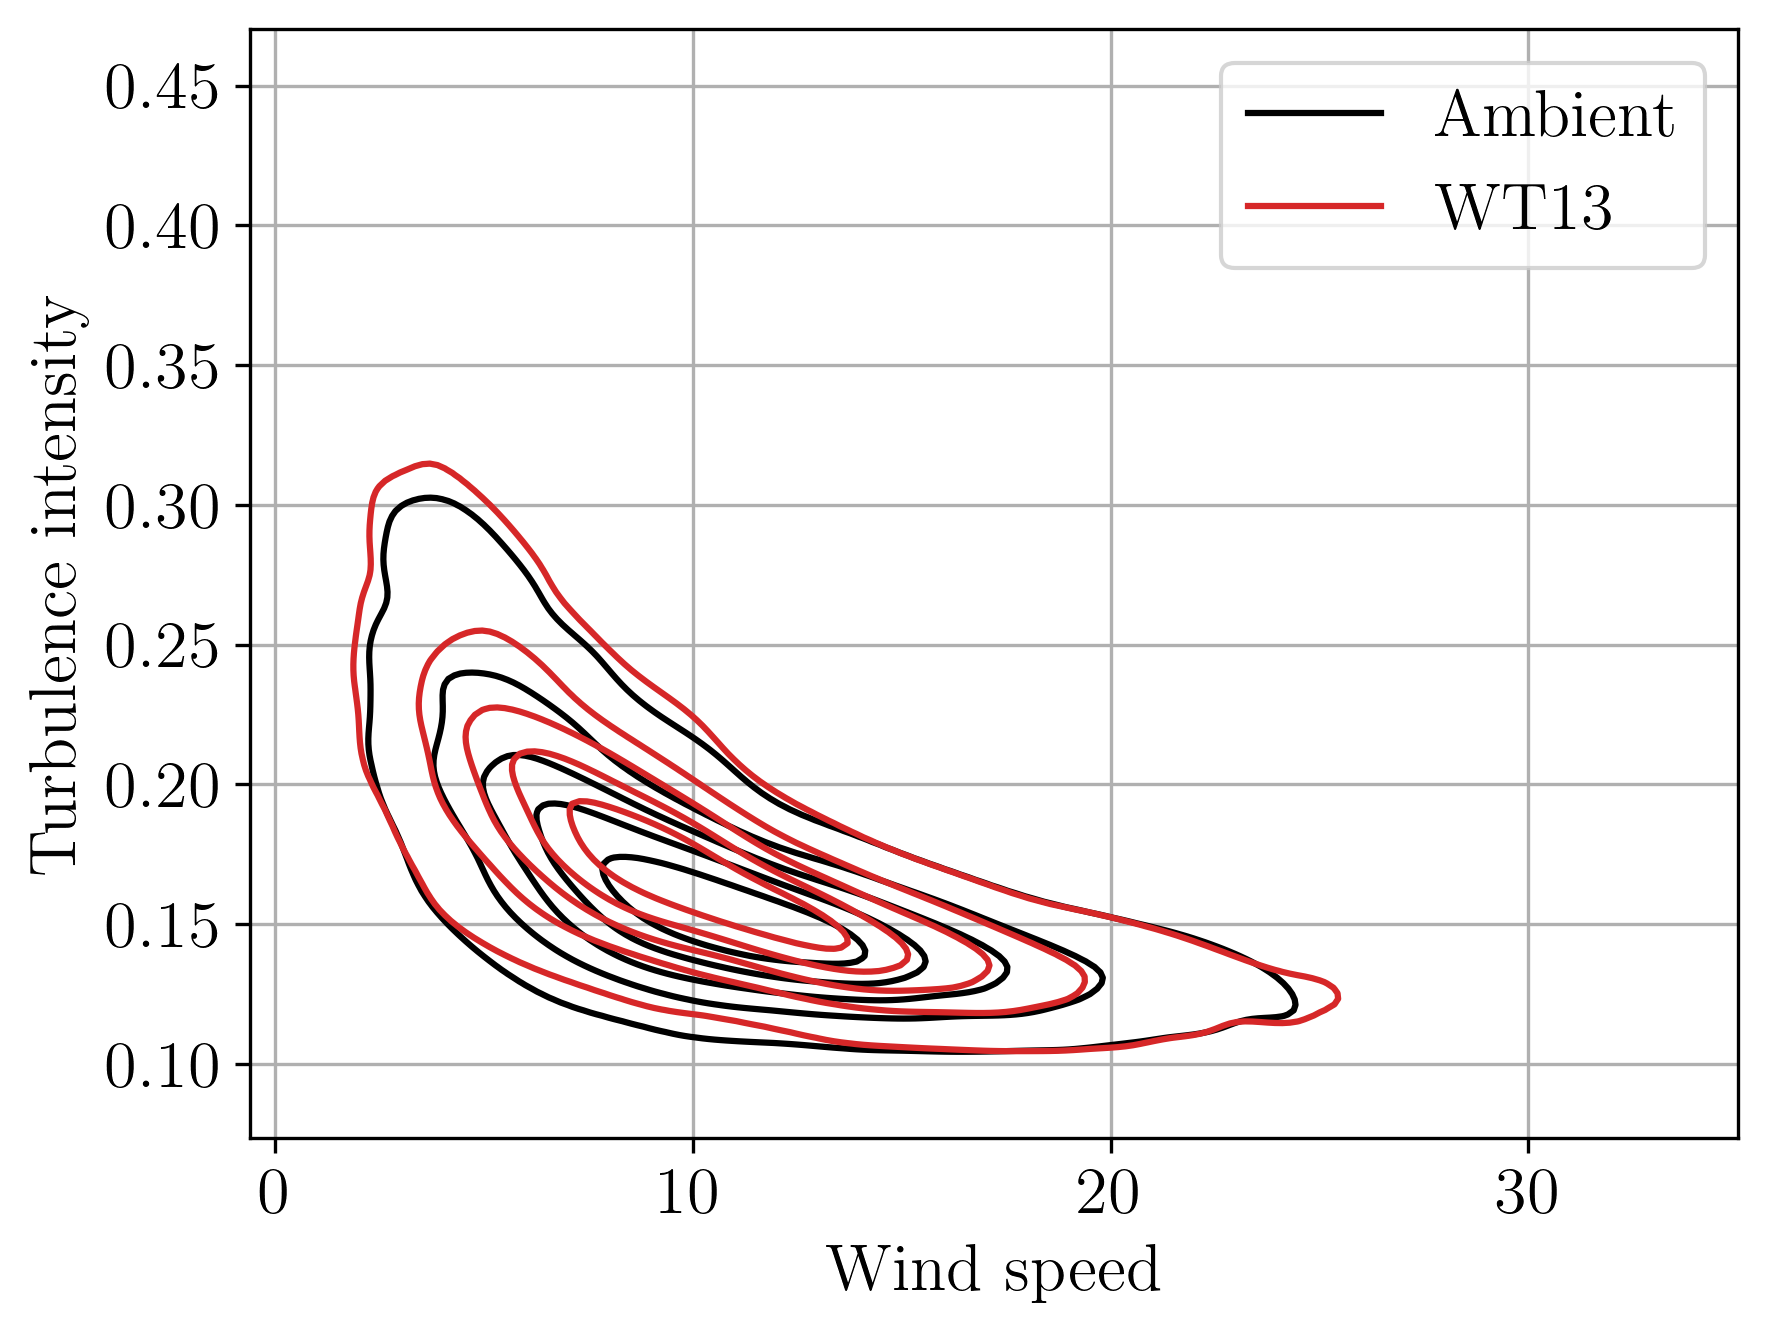
\includegraphics[width=\textwidth]{part2/figures/WAKE/joint_perturbation_SB_WT13.png}
    \end{subfigure}
    \begin{subfigure}[b]{0.3\textwidth}
        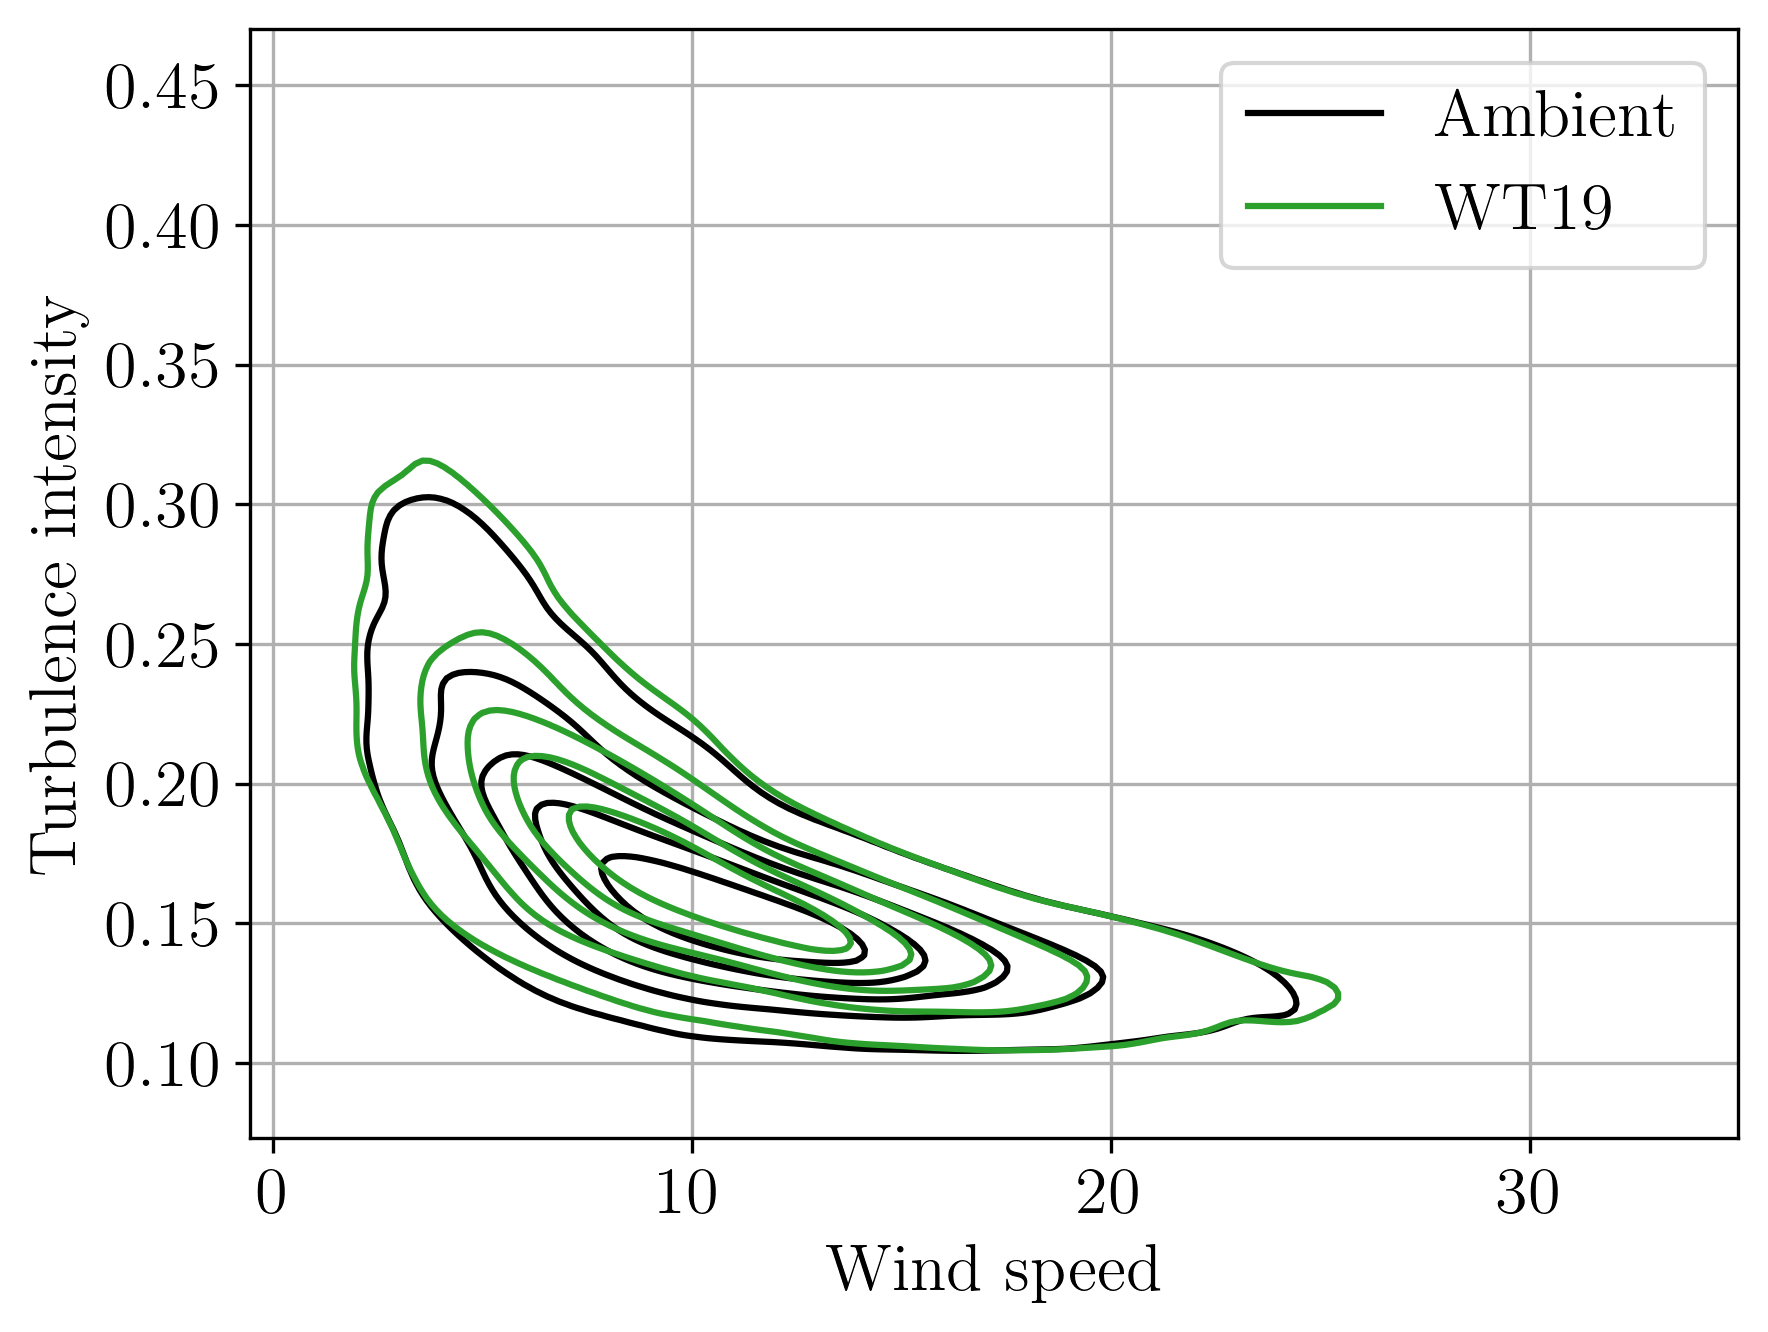
\includegraphics[width=\textwidth]{part2/figures/WAKE/joint_perturbation_SB_WT19.png}
    \end{subfigure}
    \begin{subfigure}[b]{0.3\textwidth}
        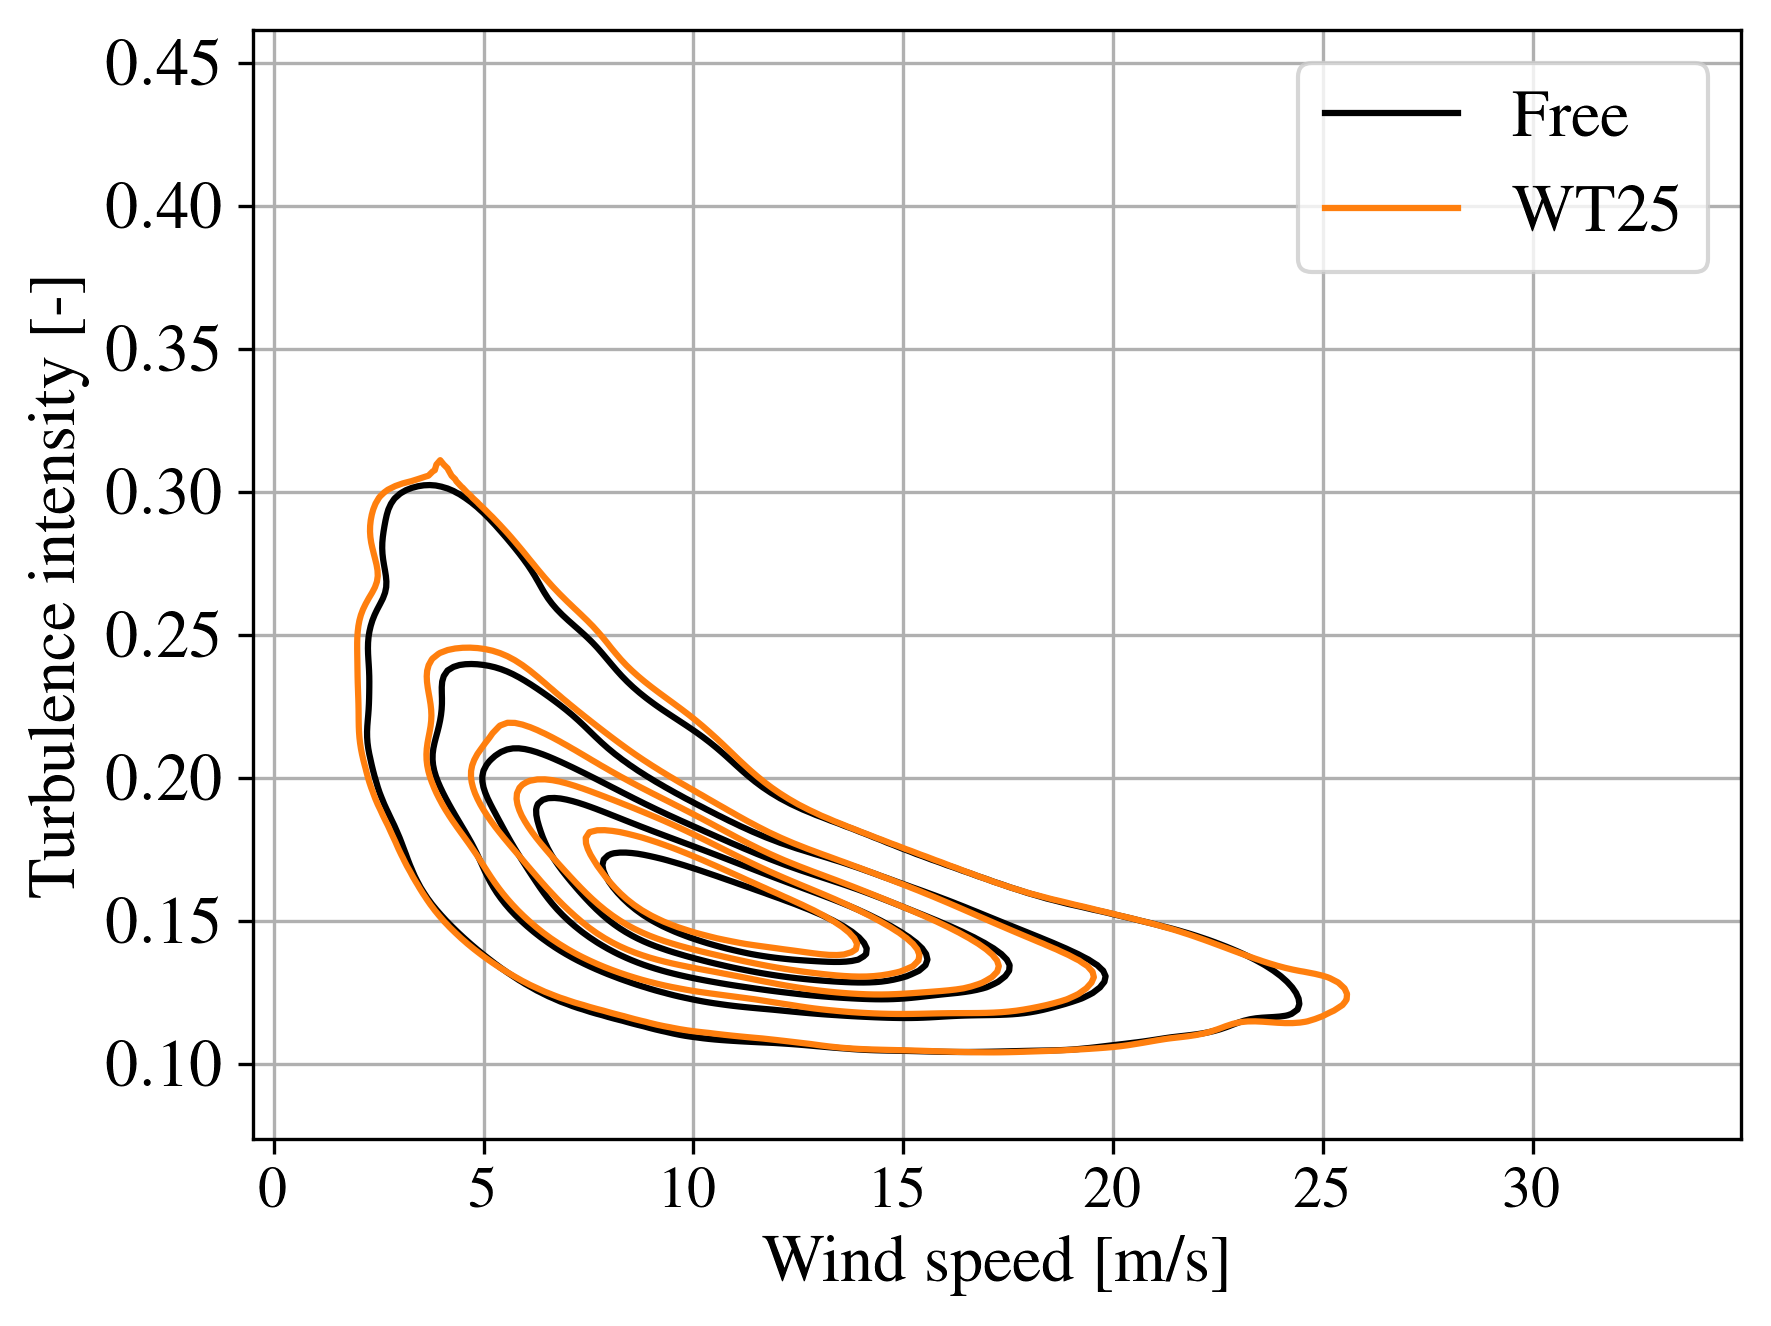
\includegraphics[width=\textwidth]{part2/figures/WAKE/joint_perturbation_SB_WT25.png}
    \end{subfigure}
    \caption{Joint perturbation at WT 13, 19, and 25}
\label{fig:FIGJointPerturbationSB}
\end{figure}

\begin{figure}
    \centering
    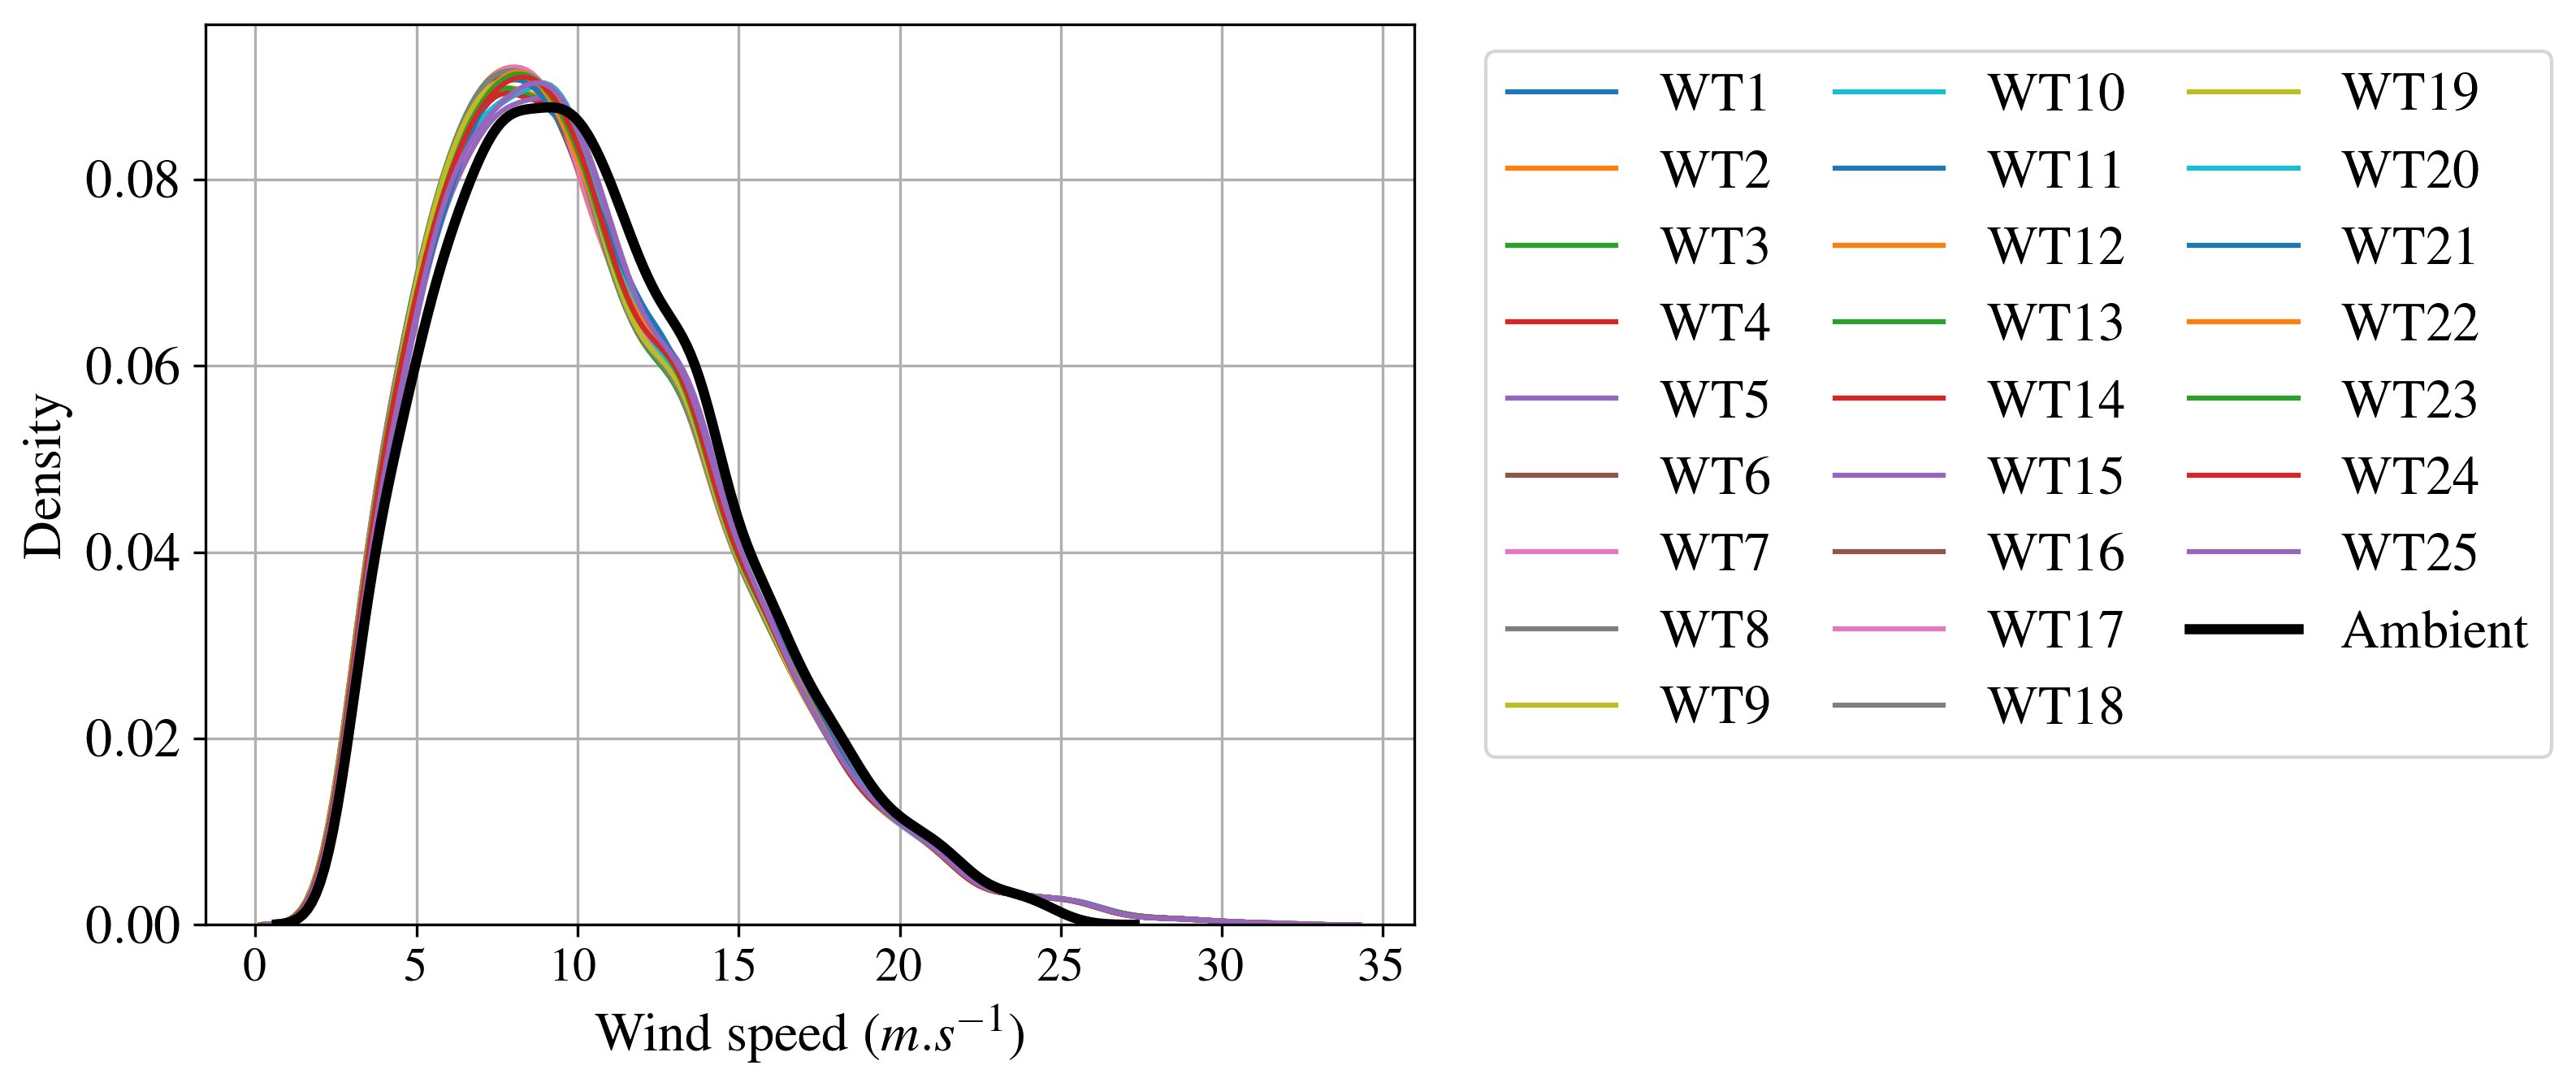
\includegraphics[width=0.7\textwidth]{part2/figures/WAKE/perturbed_wsp_distribution_SB.png}
    \caption{Ambient and wake-disturbed distributions of the wind speed}
\label{FIGMarginalWSP}
\end{figure}

\begin{figure}
    \centering
    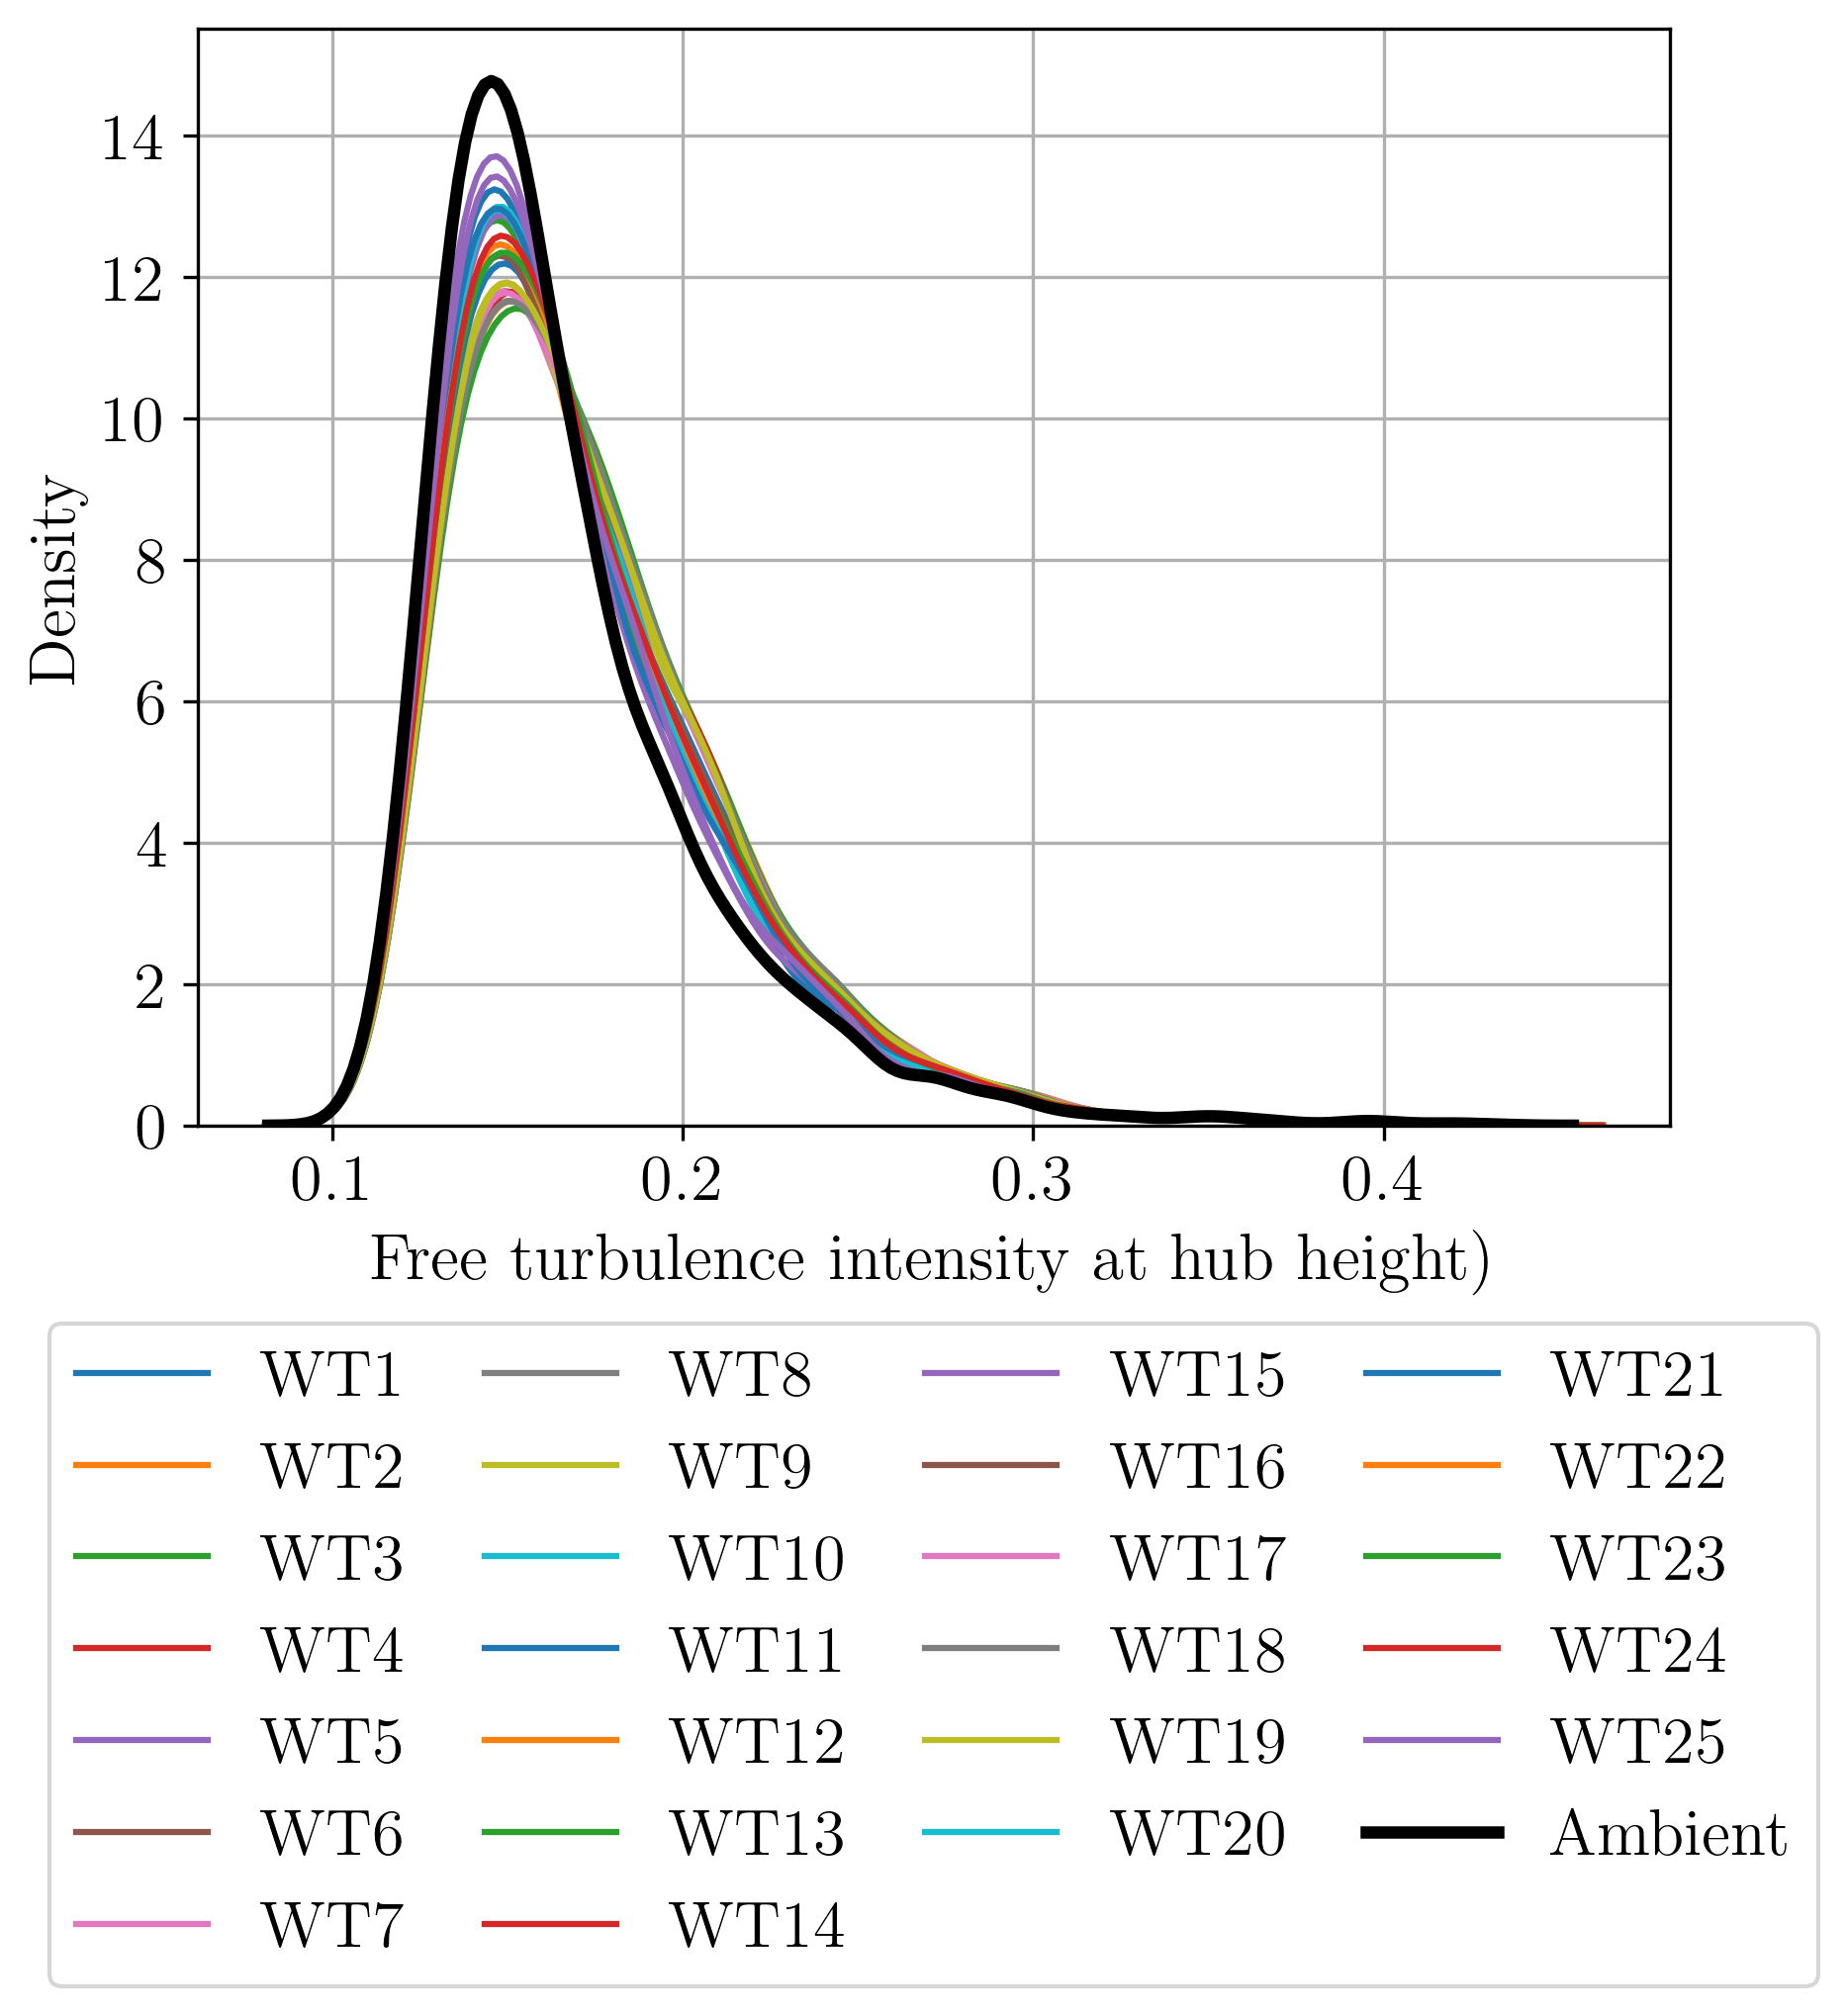
\includegraphics[width=0.7\textwidth]{part2/figures/WAKE/perturbed_ti_distribution_SB.png}
    \caption{Ambient and wake-disturbed distributions of the turbulence intensity}
\label{FIGMarginalTI}
\end{figure}




%------------------------------------------------------------%
\subsection{Statistical metric of wake-induced perturbations}
\label{sec:metric}
%------------------------------------------------------------%

%------------------------------------------------------------%
\paragraph{Maximum mean discrepancy: a distance between distributions}
%------------------------------------------------------------%
In the literature, the maximum mean discrepancy was introduced by \cite{gretton_2006} as a statistical test to discriminate two distinct distributions. 
After further work on this tool, authors such as \cite{sriperumbudur_2010} showed that the MMD is a distance between two distributions embedded in a specific function space. 
Therefore, this concept relies on the embedding of distributions in a convenient Hilbert space.
Considering a positive-definite kernel $k:\mathbb{R}^d \times \mathbb{R}^d \xrightarrow{} \mathbb{R},d \in \mathbb{N}$ 
generating a unique Hilbert space $\iH_k$ of functions equipped with inner products $ <\cdot,\cdot >_{\iH_k}$ and norms $\| \cdot \| _{\iH_k}$ (also called Reproducing Kernel Hilbert 
Space (RKHS) when the function $k(\bx,\cdot )$ satisfies the reproducing property). 
Then, let us define the kernel mean embedding of the distribution $P$ in the function space $\iH_k$:
\begin{equation}
\mu_P (\bx):=\int_{\mathbb{R}^d}{k(\bx, \by) \mathrm{d}P(\by) } \approx \frac{1}{n} \sum_{i=1}^{n}{k(\bx,\bx^{(i)})},\, \bx^{(i)} \in \bX_n.
\end{equation}
The kernel mean embedding is approximated on sample $\bX_n=(\bx^{(1)},..,\bx^{(n)})$ following the distribution $P$.
Figure \ref{fig:kernel_embedding} illustrates the kernel mean embedding of two distributions in the function space $\iH_k$ defined previously. 
Notice that this procedure allows us to embed continuous distributions (such as $P$) as well as discrete distributions (such as $Q$).

\begin{figure}[h]
    \centering
    \begin{tikzpicture}[thick, scale=0.7, every node/.style={transform shape}]
    % Axes
    \def\x{6}\def\y{3.5}
    \draw[-] (-0.5,0) -- (\x+0.5,0) node[right] {};
    \draw[-] (0,-0.5) -- (0,\y+0.5);

    \node (A) at (1.5, 3) {};
    \node (B) at (3.5, 1) {};
    \node (C) at ($(A)!0.5!(B)$) {};
    \draw[{|-|}, very thick] (A) -- (B);

    \fill [red!80] (A) circle (2pt) node[above, black] {$\mu_{P}$};
    \fill [red!80] (B) circle (2pt) node[below, black] {$\mu_{Q}$};
    \node (MMD) at (4.5, 3.5) {$\left\lVert \mu_{P} - \mu_{Q}\right\lVert_{\iH(k)}$};
    \draw[-stealth] (MMD) to [bend left] (C);

    \node [inner sep=0pt] (disc) at (-2,0.9) {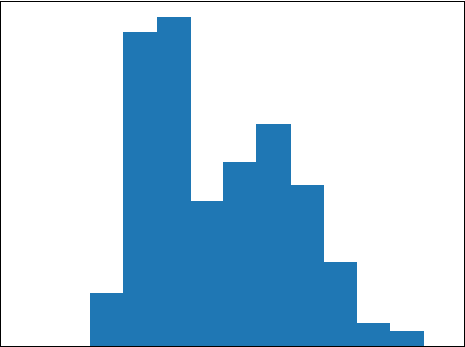
\includegraphics[width=.2\textwidth]{part2/figures/WAKE/discrete.pdf}};
    \node [inner sep=0pt] (cont) at (-2,3.1) {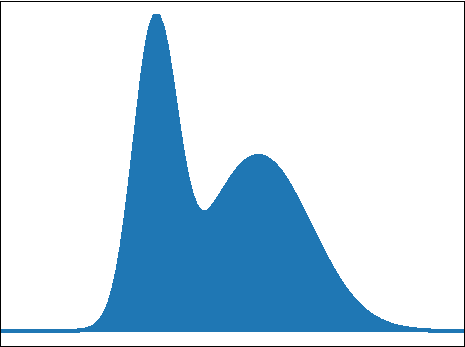
\includegraphics[width=.2\textwidth]{part2/figures/WAKE/continuous.pdf}};
    \draw[-stealth] (cont) to [bend left] (A);
    \draw[-stealth] (disc.east) to [bend right] (B);
    % Text
    \node at (5, 0.25) {$\mathcal{H}_k$};
    \node at (-3, 3) {$P$};
    \node at (-3, 1) {$Q$};
\end{tikzpicture}
    \caption{Kernel mean embedding of two probability distributions $P$ and $Q$ mapped in the $RKHS$  $H_k$}
    \label{fig:kernel_embedding}
\end{figure}

The distance between the two kernel mean embeddings $\mu_P$  and $\mu_Q$ is called the maximum mean discrepancy (MMD). 
This distance between two distributions $P$ and $Q$ is initially defined by the worst-case error for any function within a unit ball of a Hilbert space $\iH_k$, generated by the kernel $k$:

\begin{equation}
\mathrm{MMD}_k(P,Q):=\underset{\| g \|_{\iH_k} \leq 1}{\mathrm{sup}} 
\left\lvert \int_{\mathbb{R}^d}{g(\bx) \mathrm{d}P(\bx)}
- \int_{\mathbb{R}^d}{g(\bx) \mathrm{d}Q(\bx)} \right\rvert
= \|\mu_P(\bx) - \mu_Q(\bx) \| _ {\iH_k}.
\end{equation}
The MMD fully relies on the difference of kernel mean embeddings. 
Moreover, according to \cite{sriperumbudur_2010}, a kernel is called “characteristic kernel” when the following equivalence is true, $MMD_k (P,Q)=0 \iff P=Q$, making the MMD a metric on $\mathbb{R}^d$. 
For its good convergence behavior, the squared MMD has been used for multiple other purposes than numerical integration: statistical testing \cite{gretton_2006}, sensitivity analysis \cite{daveiga_2015}. 
When elevated to the square, it can be estimated using one $n$-sized representative sample of $P$ denoted $\left\{ \bx^{(i)} \right\}_{i \in (1,..,n)}$
(and respectively one $m$-sized sample of $Q$ denoted $\left\{ \by^{(i)} \right\} _{i \in (1,..,m)}$:

\begin{equation}
\widehat{\mathrm{MMD}_k}(P,Q) ^ 2 = \frac{1}{n^2} 
\sum_{i,j=1}^{n}{k(\bx^{(i)}, \bx^{(j)})} - \frac{2}{n m} \sum_{i=1}^{n}{ } \sum_{j=1}^{m}{k(\bx^{(i)},\by^{(j)})} + \frac{1}{m^2}  \sum_{i,j=1}^{m}{k(\by^{(i)},\by^{(j)})}.
\end{equation}
In the following, the idea is to compare the ambient wind distribution $p_0$ to the wake-perturbed wind conditions $p_l'$ at the WT~$l$ using the previously defined squared MMD.

%------------------------------------------------------------%
\paragraph{Application to the South Brittany wind farm project}
\label{SecApplicationSB}
%------------------------------------------------------------%
Once the joint perturbed distributions of each WT are estimated by a large Monte Carlo sample (cf. section~\ref{sec:UQ-wake}), the MMD with the ambient wind conditions can be computed. 
Figure~\ref{FIGWakeEffect} illustrates for each WT the squared MMD value computed to measure the wake-induced perturbation. 
Let us remind that MMD is a distance between the joint perturbed distribution at a WT computed for all wind orientations with the ambient wind distribution. 
Despite the wake obviously depend on the wind direction, our final goal is to define a small number of WT for RBD thus independently of the wind orientation. 
The lower this metric gets, the closer to the ambient wind distribution. 
Quite logically, the WT in the center of the farm are more affected by the wake since they are subject to the wake regardless of the wind direction.

The values of squared MMD given in the previous figure are estimated between two samples:
\begin{itemize}
    \item the Monte Carlo sample of the free environmental distribution: $\bX_n$,
    \item the wake-perturbed Monte Carlo sample at the WT $l: \bX'_{n,l}$ (output of the steady-state wake numerical model).
\end{itemize}

To ensure that the Monte-Carlo estimation converged, Figure~\ref{FIGConvergenceMMD} plots the squared MMD between the sample $\bX_n$ and the increasing samples $\bX'_{i,l},i \in {400,..,6000}$. 
After a few thousands of simulations, the MMD of each WT tends to converge towards a stable value, as expected. 
The design of experiment with $n=6~000$ is thus considered as sufficient. 

\begin{figure}
    \centering
    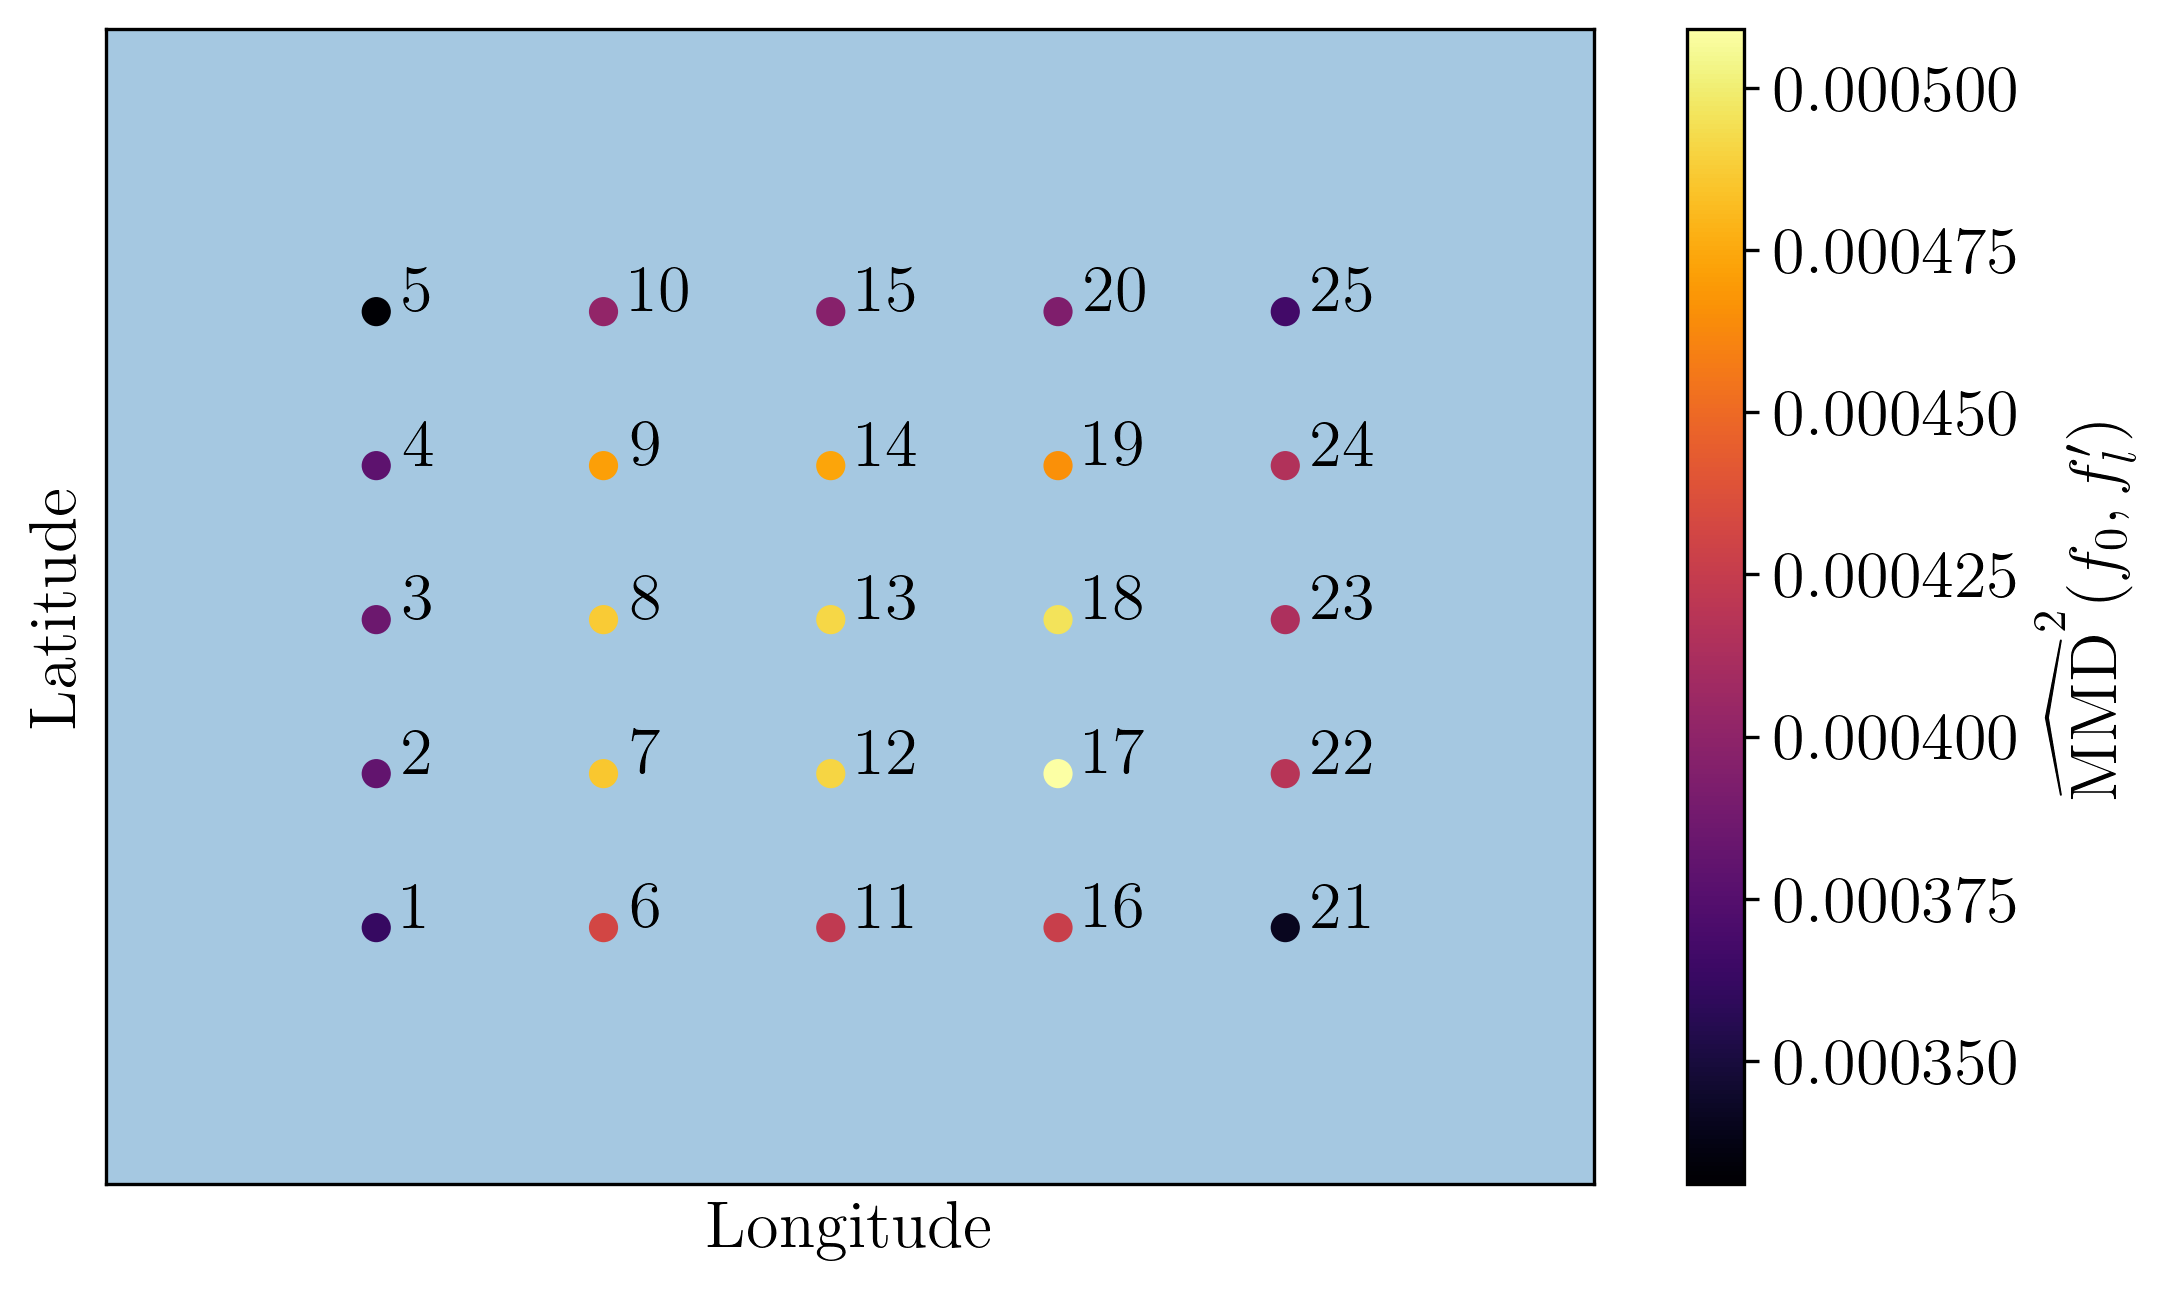
\includegraphics[width=0.6\textwidth]{part2/figures/WAKE/wake_perturbation_SB.png}
    \caption{South Brittany layout and wake effects measured by the squared MMD on wind conditions. 
    Note that the vertical direction on this plot does not represent the north direction.}
\label{FIGWakeEffect}
\end{figure}

\begin{figure}
    \centering
    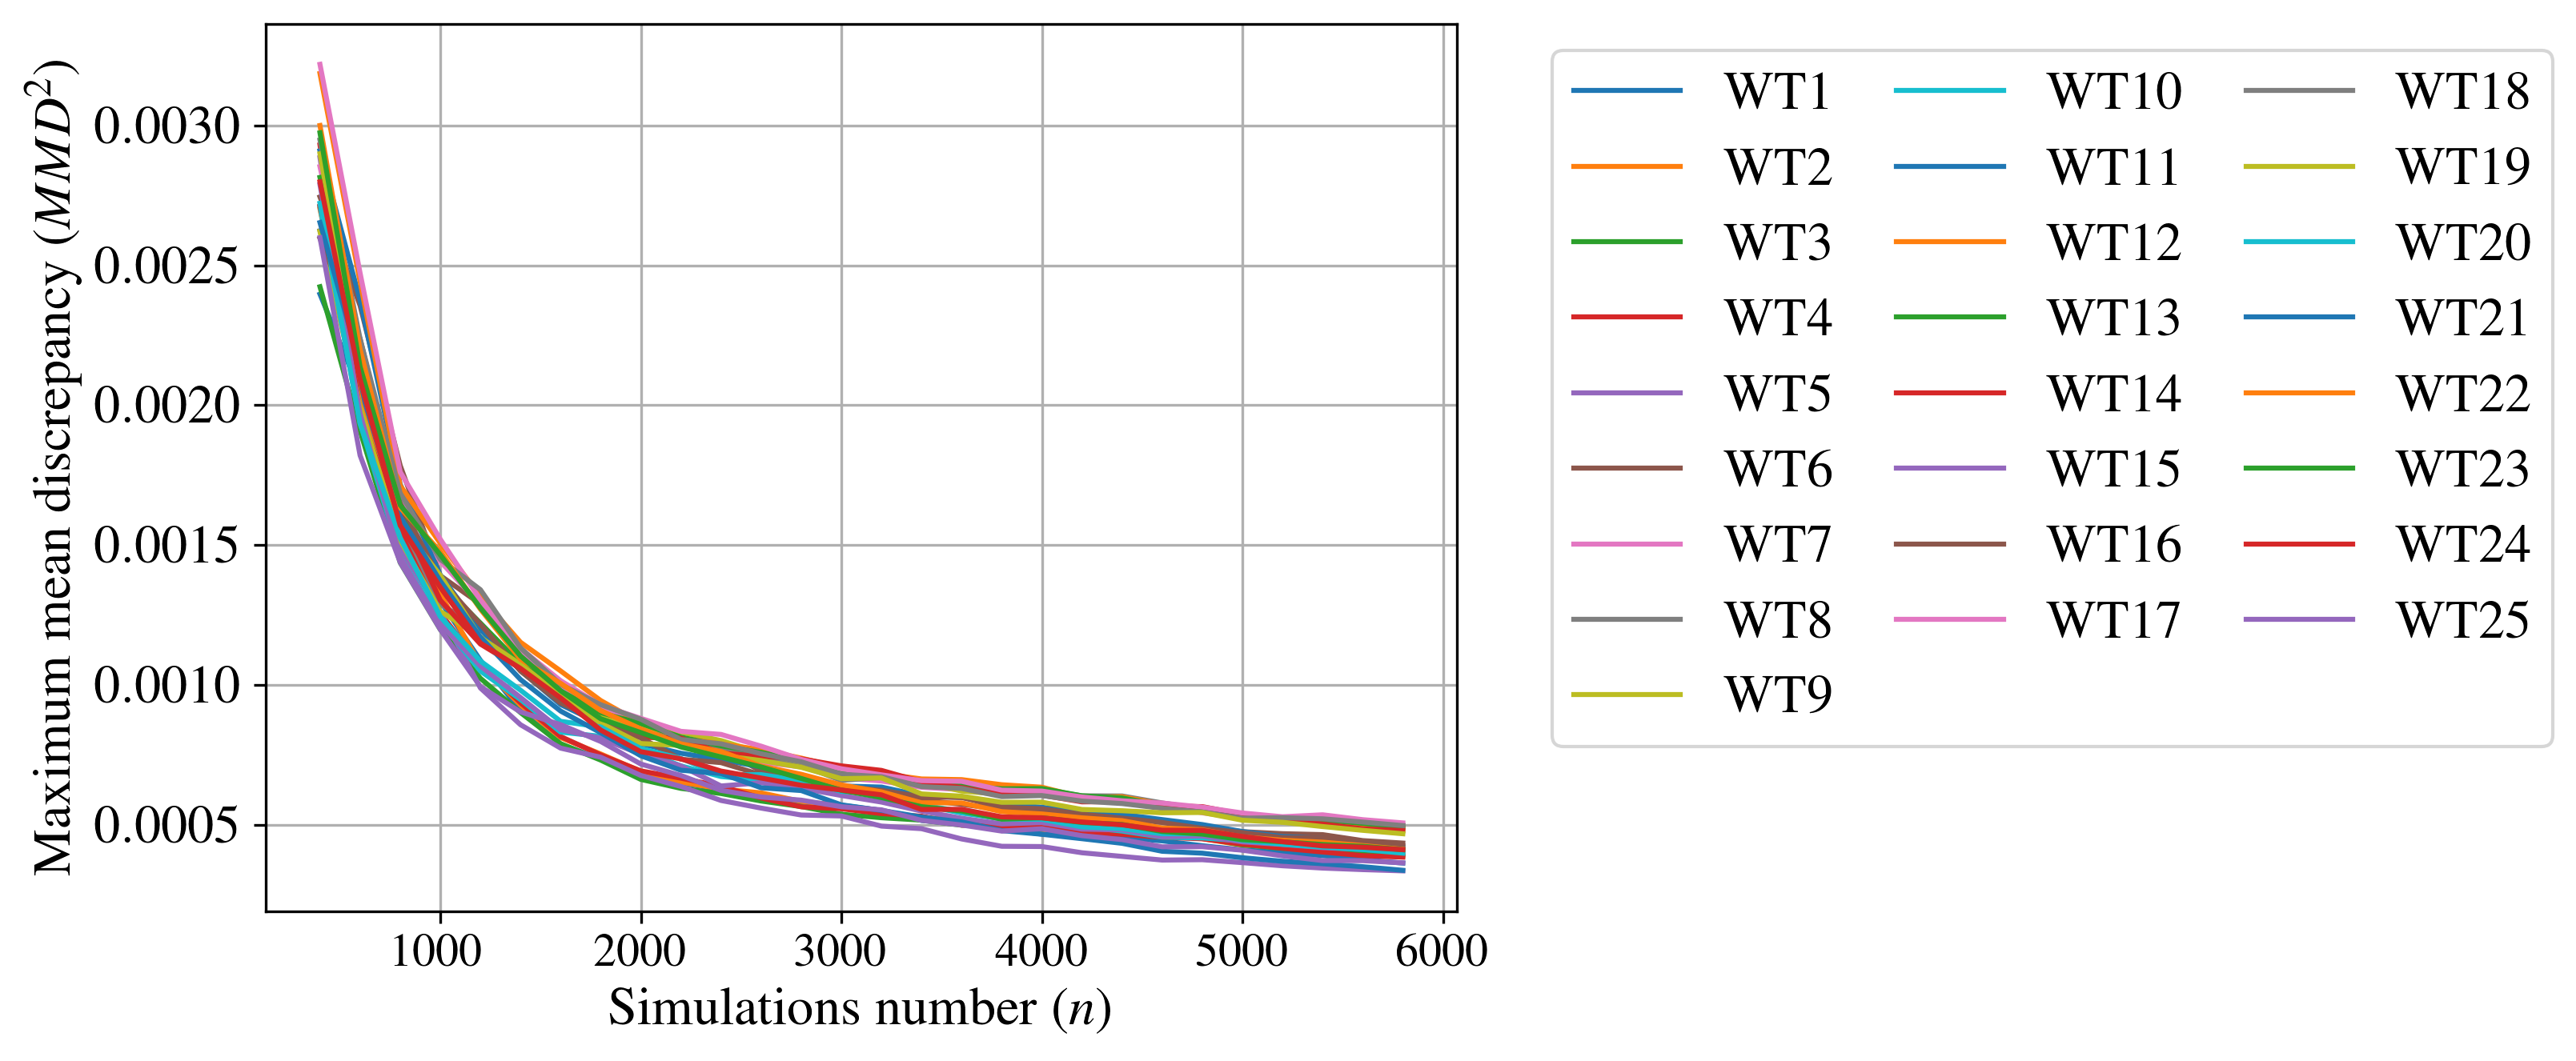
\includegraphics[width=0.7\textwidth]{part2/figures/WAKE/convergence_MC_SB.png}
    \caption{Convergence of the squared MMD estimation}
\label{FIGConvergenceMMD}
\end{figure}

%------------------------------------------------------------%
\subsection{Conclusion}
%------------------------------------------------------------%
A steady-state engineering wake model is coupled with a hydrostatic solver to take into account the effect of the floaters position in the wake computation of a floating offshore wind farm
The main impact of the floater's position is the increased rotor tilt, which leads to a larger vertical deflection of the wake. 
In the South-Brittany farm, the elevation of wake center is significant and could modify the fatigue loads on the downstream WT. 
This low-fidelity, or engineering model is very fast (about 3 minutes on a regular computer), while higher fidelity models can simulate the wake in a wind farm more accurately, but with much higher computational cost (several days for LES Meso-NH solver, with intensive parallelisation). 
In this paper, we consider that the modelling error made by the engineering wake model as reasonable. 
Further investigations should be done on the integration of the different fidelity levels in the uncertainty propagation. 
In this work, the uncertainty propagation is performed for to random inputs: the wind speed and the turbulence intensity, leading to a wake perturbed distribution per WT. 
A metric was then defined to measure the distance between distributions in order to build clusters of WT seeing similar wind conditions. 
After applying the metric to the South Brittany case, a clustering approach is used to determine a limited number of WTs representing the farm for RBD. 
Several clustering methods are compared and provide similar results for the current case study. In this case, a solution with 4 clusters is a good compromise between low relative error with clusters and low number of clusters. 
Getting a low number of clusters allows us to reduce the number of representative WT on which a RBD study can be done to assess the RBD over the whole farm. 
The differences among a cluster and between clusters have to be studied when looking directly to the output of interest for ultimate or fatigue reliability. 
However the difference on load output quantities may be reduced when compared to that on wake output quantities thanks to the damping of the WT. 
Depending on the definition of a wind farm failure (series system: one WT fails or parallel system: all WT fail or intermediate system), the probability of failure can be estimated from the probability of failure of the representative WT. 
These considerations need to be further explored to improve RBD at the farm scale. 


%============================================================%
\section{Conclusion}
%============================================================%